\documentclass[a4paper,11pt]{article}
\usepackage[UKenglish]{babel}
\usepackage[table]{xcolor}
\usepackage{graphicx}
\usepackage{courier}
\usepackage{color}
\usepackage{array}
\usepackage{pstricks}
\usepackage{parskip}
\usepackage[bottom]{footmisc}
\usepackage{fancyhdr}
\usepackage{multirow}
\usepackage{longtable}
\usepackage{siunitx}
% the hyperref package must always be the last package to be included
\usepackage[pdftex,
            pdfusetitle,
            pdfsubject={Technical Reference Manual for dastaZ80 homebrew computer},
            pdfkeywords={Z80, homebrew computer, Operating System, OS, programmer, technical, reference, manual}
        ]{hyperref}

\hypersetup{
    colorlinks = true,
    linkcolor = blue,
    anchorcolor = blue,
    citecolor = blue,
    filecolor = blue,
    urlcolor = blue
}

\setlength\parindent{0pt}

\begin{document}
    \pagestyle{empty}
    % ==========================================================================
    % Cover page
    % ==========================================================================
    \begin{pspicture}(8.5,11)
        \rput[b](3.5,8){
            \parbox{7in}{
                \begin{flushright}
                    \Huge\bfseries\sffamily dastaZ80 Mark II\\ Technical Reference Manual
                \end{flushright}
            }
        }
        \uput[0](0,0){\color{blue}\rule{7in}{0.5ex}}
    \end{pspicture}
    \title{dastaZ80 Technical Reference Manual}
    \author{David Asta}
    \date{11 October 2022}

    \pagebreak
    % ==========================================================================
    % Header & Footer
    % ==========================================================================
    \pagestyle{fancy}
    \fancyhf{}
    \fancyhead[R]{dastaZ80 Mark II Technical Reference Manual}
    % ==========================================================================
    \section*{Disclaimer}
    % ==========================================================================
    The products described in this manual are intended for educational purposes,
    and should not be used for controlling any machinery, critical component in
    life support devices or any system in which failure could result in personal
    injury if any of the described here products fail.
    
    These products are subject to continuous development and improvement. All
    information of a technical nature and particulars of the products and its
    use are given by the author in good faith. However, it is acknowledged that
    there may be errors or omissions in this manual. Therefore, the author
    cannot accept any liability for any loss or damage arising from the use of
    any information or particulars in this manual.

    % ==========================================================================
    \section*{Licenses}
    % ==========================================================================
    \small
    \textbf{Hardware} is licensed under the \textbf{Creative Commons
    Attribution-ShareAlike 4.0 International License}
    
    \hspace{1cm}http://creativecommons.org/licenses/by-sa/4.0/
    
    \textbf{Software} is licensed under \textbf{The MIT License}
    
    \hspace{1cm}https://opensource.org/licenses/MIT
    
    \textbf{Documentation} is licensed under the \textbf{Creative Commons
    Attribution-ShareAlike 4.0 International License}
    
    \hspace{1cm}http://creativecommons.org/licenses/by-sa/4.0/

    \normalsize

    \hrulefill

    \textcopyright 2022 David Asta

    \pagebreak
    % ==========================================================================
    \section*{Document Conventions}
    % ==========================================================================
    The following conventions are used in this manual:

    \begin{center}
        \begin{tabular}{c m{9cm}}
            \hline
            \textbf{DEVICE} & Device names are displayed in bold all upper case 
            letters, and refer to hardware devices.\\
            \hline
            \texttt{Courier} & Text appearing in the \texttt{Courier} font 
            represents either an OS System Variable a Z80 CPU Register
            or a Z80 Flag. OS System Variables are identifiers for specific
            \textbf{MEMORY} addresses that can be used to read statuses and to
            pass information between routines or programs.\\
            \hline
            \texttt{0x14B0} & Numbers prefixed by 0x indicate an Hexadecimal value.
            Unless specified, memory addresses are always expressed in
            Hexadecimal.\\
            \hline
        \end{tabular}
    \end{center}

    The SD card is referred as \textbf{DISK}.

    The Floppy Disk Drive is referred as \textbf{DISK} or as \textbf{FDD}.

    The 80 column text VGA output is referred as \textbf{CONSOLE} or as
    \textbf{High Resolution Display}.

    The 40 column graphics Composite Video output is referred as \textbf{Low
    Resolution Display}.

    The Operating System may be referred as DZOS, dzOS or simply OS.

    \textbf{MEMORY} refers to both \textbf{ROM} and \textbf{RAM}.

    Memory used by the \textbf{Low Resolution Display} is referred as
    \textbf{VRAM} (Video RAM).

    \pagebreak
    % ==========================================================================
    \section*{Related Documentation}
    % ==========================================================================
    \begin{itemize}
        \item dastaZ80 User's Manual\cite{dastaz80userman}
        \item dastaZ80 Programmer's Reference Guide\cite{dastaz80progref}
        \item dzOS Github Repository\cite{dastaZ80github}
    \end{itemize}

    \pagebreak
    % ==========================================================================
    \tableofcontents
    % ==========================================================================

    \pagebreak
    % ==========================================================================
    % Header & Footer
    % ==========================================================================
    \pagestyle{fancy}
    \fancyhf{}
    \fancyhead[R]{dastaZ80 Mark II Technical Reference Manual}
    \fancyfoot[R]{\thepage}
    \setcounter{page}{1}

    % ==========================================================================
    \section{Boards and Case}
    % ==========================================================================

    The final aim of dastaZ80 is to be a single board computer, but at the 
    moment I am making small \textit{module boards} so that I can test and 
    troubleshoot independently. Plus it allows me to easily upgrade and test
    (e.g. when I changed the serial board from a MC68B50 ACIA to a Zilog SIO/2).

    % ==========================================================================
    \subsection{Main board}
    % ==========================================================================

    This board is the heart of the computer, and contains the CPU chip, the 
    clock circuit, the reset circuit, the ROM chip, the RAM chip, the I/O
    decoding logic and the memory decoding logic.

    % ==========================================================================
    \subsubsection{CPU}
    % ==========================================================================

    The CPU is a Zilog Z80 (Z0840006PSC) NMOS 40-pin plastic DIP, rated at 6.17
    Mhz, but overclocked to 7.3728 MHz.

    The signals \textit{/INT}, \textit{/BUSREQ},\textit{/WAIT} and \textit{/NMI}
    are connected to 10K pull-up resistor

    % ==========================================================================
    \subsubsection{Clock circuit}
    % ==========================================================================

    This is the system clock, running at 7.3728 MHz, that drives the CPU and the
    SIO/2 Channels. It is a very simple circuit consisting of a crystal
    oscillator and a copule of resistors and ceramic capacitors.

    % ==========================================================================
    \subsubsection{Reset circuit}
    % ==========================================================================
    
    After power up, the CPU needs to be reset, through the \textit{/RESET}
    signal. When this signal is low for a minimum of three full clock cycles,
    the CPU resets the interrupt enable flip-flop, clears the Program Counter
    (\texttt{PC}), clears registers \texttt{I} and \texttt{R}, and sets the
    interrupt status to Mode 0. 

    In the dastaZ80, the reset circuit is a bit more complicated than the 
    typical reset circuit found in homebrew computers. The reason is that the
    VGA output is done with a LILYGO TTGO  VGA32 V1.4\footnote{An ESP32 board
    with a VGA output, that runs FABGL to provide an ANSI terminal.}, which
    needs a few seconds to initialise. So the reset is hold for 6.5 seconds, to
    allow the initialisation to finish,  and then reset the CPU and rest of
    devices.

    Using an NE555 timer running in monostable mode, the \textit{/RESET} signal
    is kept low a number of seconds that can be deduced with the formula: 
    $T = 1.1 * R2 * C2$. (e.g. $1.1 * 270000 (270K) * 0.000022 (22\mu F) = 
    6.534 seconds$).

    \begin{center}
        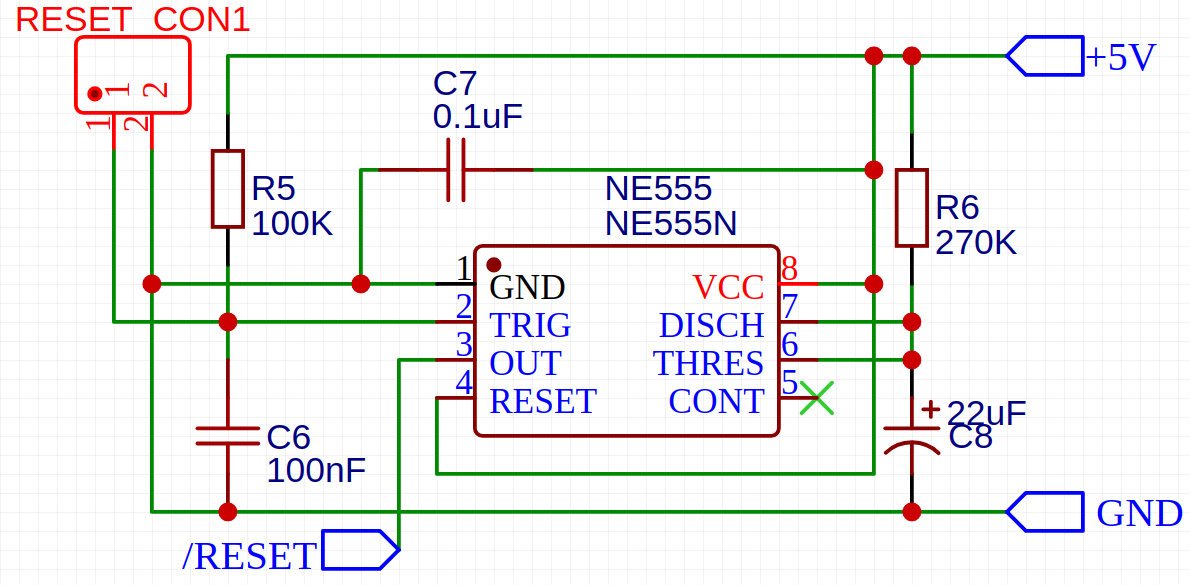
\includegraphics[scale=0.3]{dastaz80resetcircuit.png}
    \end{center}

    The \textit{RESET\_CON1} is connected to a push-button. R5 and C1 are used as 
    anti-debounce for the button.

    % ==========================================================================
    \subsubsection{ROM chip}
    % ==========================================================================

    The ROM chip is a Winbond W27E512 (64K x 8 bit) EEPROM (Electrically Erasable
    Programmable Read-Only Memory) 28-pin plastic DIP, mnounted on a ZIF (Zero
    Insert Force) socket for easy extraction/insertion for programming.

    The signal \textit{A15} is connected to \textit{+5V}, therefore is always
    high, meaning that the start address is \texttt{0x8000} and the ROM becomes
    a 32 KB ROM. This is not the start address that the CPU sees but rather the
    address where the ROM starts. The CPU will see it as \texttt{0x0000}.

    As the dzOS is 16 KB in size, I have divided the ROM into two 16 KB ROMs, 
    allowing to execute two different operating systems by selecting the start
    address (\texttt{0x8000} or \texttt{0xC000}) via a switch connected to the
    signal \textit{A14} of the ROM chip.

    When the switch is in the lower position, \textit{A14} is connected to 
    \textit{Ground}, thus start address \texttt{0x0000} starts at 
    \texttt{0x8000} in the ROM. When the switch is in the upper position, 
    \textit{A14} is connected to \textit{+5V}, thus start address is at 
    \texttt{0xC000}.

    The idea is to be able to use the computer with either dzOS or Digital 
    Research, Inc. CP/M. Of course, the SD will need to be changed for the
    specific operating system.

    % ==========================================================================
    \subsubsection{RAM chip}
    % ==========================================================================

    The RAM is an AS6C1008 (128K x 8 bit) CMOS SRAM 32-pin plastic DIP.

    As the Z80 can only address 65,536 bytes (64 KB), \textit{A16} on this chip
    is connected to \textit{Ground}, therefore it will always be low, and hence
    only 65,536 bytes (64 KB) are available.

    % ==========================================================================
    \subsection{ Arduino Serial Multi-Device Controller (ASMDC)}
    % ==========================================================================

    An Arduino board acting as a \textit{man-in-the-middle} to dastaZ80 to
    communicate with different devices like Real-Time Clock, NVRAM, SD card,
    Floppy Disc Drive, and more.

    The dastaZ80's SIO/2 Channel B is connected to an Arduino Mega2560's serial
    port. The dastaZ80 sends commands (identified by a unique single byte) to
    the Arduino, which interprets the received command and communicates with the
    corresponding attached device (e.g. get time from the RTC), and send
    information back to the dastaZ80.

    % ==========================================================================
    \subsubsection{Floppy Disk Drive (FDD)}
    % ==========================================================================

    This module is connected to original Acorn A3010 FDD (Citizen OSDA-20C).

    The available commands (cmd) are:
 
     \begin{tabular}{| c | m{3.8cm} | m{3cm} | m{3.5cm} | }
         \hline
         \rowcolor{lightgray}
         cmd & Description & (Size) Input & (Size) Output\\
         \hline
         A0 & FDD Status & (0) & (1) see below\\
         \hline
         A1 & FDD Busy & (0) & (1) 0x00=Not Busy\\
            &          &     &     0x01=Busy\\
         \hline
         A2 & Read sector from Floppy Disk & (2) sector\_num\_lsb sector\_num\_msb & (512) Sector contents\\
         \hline
         A3 & Write sector into Floppy Disk & (512) Sector contents & (0) \\
         \hline
         A4 & Checks if a disk is in the drive & (0) & (1) 0x00=Disk is in\\
            &                                  &     &     0xFF=No disk\\
         \hline
         A5 & Checks if a disk is Write Protected & (0) & (1) 0x00=Protected\\
            &                                     &     &     0xFF=Unprotected\\
         \hline
         A6 & Set drive as Double-density & (0) & (0)\\
         \hline
         A7 & Set drive as High-density & (0) & (0)\\
         \hline
         A8 & Low-level format (nop file sustem) & (0) & (1) Return code (0=success)\\
         \hline
         AA & Turn FDD motor ON & (0) & (0)\\
         \hline
         AB & Turn FDD motor OFF & (0) & (0)\\
         \hline
     \end{tabular}

     \textbf{A0 (FDD Status)}

     Tells the status of the FDD.\\

     This command should be called after each command on the \textbf{FDD} to
     check if the command was successful or not. Any value other than
     \texttt{0x00} indicates and error.

     \begin{itemize}
        \item \textbf{Lower Nibble} (\texttt{0x00} if all OK)
        \begin{itemize}
            \item \textbf{bit 0} = not used
            \item \textbf{bit 1} = not used
            \item \textbf{bit 2} = set if last command resulted in error
            \item \textbf{bit 3} = not used
        \end{itemize}
        \item \textbf{Upper Nibble} (error code)
    \end{itemize}

    % ==========================================================================
    \subsubsection{Micro SD Card Module}
    % ==========================================================================

    This module is connected to the Arduino via SPI.

    The available commands (cmd) are:

    \begin{tabular}{| c | m{3.8cm} | m{3cm} | m{3.5cm} | }
        \hline
        \rowcolor{lightgray}
        cmd & Description & (Size) Input & (Size) Output\\
        \hline
        B0 & SD Card status & (0) & (1) see below\\
        \hline
        B1 & SD Card Busy & (0) & (1) 0x00=Not Busy\\
           &              &     &     0x01=Busy\\
        \hline
        B2 & Read sector from Image in SD Card & (2) sector\_num\_lsb sector\_num\_msb & (512) Sector contents\\
        \hline
        B3 & Write sector into Image in SD Card & (512) Sector contents & (0) \\
        \hline
        B4 & Close Image File & (0) & (0)\\
        \hline
        B5 & Open Image File & (0) & (0)\\
        \hline
    \end{tabular}

    \textbf{B0 (SD Card Status)}

    Tells the status of the SD Card reader.\\

    This command should be called after each command on the \textbf{SD card} to
    check if the command was successful or not. Any value other than
    \texttt{0x00} indicates and error.

     \begin{itemize}
        \item \textbf{Lower Nibble} (\texttt{0x00} if all OK)
        \begin{itemize}
            \item \textbf{bit 0} = set if \textbf{SD card} was not found
            \item \textbf{bit 1} = set if image file was not found
            \item \textbf{bit 2} = set if last command resulted in error
            \item \textbf{bit 3} = not used
        \end{itemize}
        \item \textbf{Upper Nibble} (number of disk image files found)
    \end{itemize}

    % ==========================================================================
    \subsubsection{Real-Time Clock (RTC) Module}
    % ==========================================================================

    The RTC is a DS3231 module connected to the Arduino via I2C.

    The available commands (cmd) are:

    \begin{tabular}{| c | m{3.8cm} | m{3cm} | m{3.5cm} | }
        \hline
        \rowcolor{lightgray}
        cmd & Description & (Size) Input & (Size) Output\\
        \hline
        C0 & Get RTC info & (0) & (1) see below\\
        \hline
        C1 & Check Battery Health & (0) & (1) 0xA0=Healthy\\
           &                      &     &     0x00=Dead\\
        \hline
        C2 & Get current Date (in Hexadecimal) & (0) & (9) CCYYMMDDW\\
        \hline
        C3 & Get current Time (in Hexadecimal) & (0) & (6) HHMMSS\\
        \hline
        C4 & Set Date & (7) YYMMDDW & (0)\\
        \hline
        C5 & Set Time & (6) HHMMSS & (0)\\
        \hline
    \end{tabular}

    \textbf{C0 (Get RTC info)}

    Tells information of the configuration of the \textbf{RTC} module.\\

    Useful, for example if the time is not kept accurately, to check if the
    clock is running or not.

     \begin{itemize}
        \item \textbf{Byte 1}
        \begin{itemize}
            \item \textbf{bit 0} = set if clock is running
            \item \textbf{bit 1} = set if clock is in 24 hours mode. Otherwise,
            clock is in 12 hours mode
            \item \textbf{bit 2} = set if alarm 1 is ON
            \item \textbf{bit 3} = set if alarm 2 is ON
        \end{itemize}
    \end{itemize}

     % ==========================================================================
     \subsubsection{NVRAM}
     % ==========================================================================
 
     This module is part of the Real-Time Clock module.

     This module is not currently used by dzOS.
 
     The available commands (cmd) are:
 
     \begin{tabular}{| c | m{3.8cm} | m{3cm} | m{3.5cm} | }
         \hline
         \rowcolor{lightgray}
         cmd & Description & (Size) Input & (Size) Output\\
         \hline
         D0 & Test  NVRAM can be written & (0) & (1) NVRAM capacity (in bytes) or 0xFF if failure\\
         \hline
         D1 & Clear (Set all to zeros) NVRAM & (0) & (0) \\
         \hline
     \end{tabular}

    % ==========================================================================
    \subsection{Serial board}
    % ==========================================================================

    The serial board consists of a Zilog SIO/2 (Z84C4208PEG) CMOS 40-pin plastic
    DIP, rated at 8 MHz, that offers two independent full-duplex channels for
    data serial communication.

    Channel A is used for communication with the Keyboard Interface and the VGA
    Interface. The Transmit signal (\textit{TX}) of the Keyboard Interface is
    connected to the Receive signal (\textit{RX}) of the Channel A, and the 
    Transmit signal (\textit{TX}) of the Channel A is connected to the Receive
    signal (\textit{RX}) of the VGA Interface.

    The type of implementation allows for easy replacement of the keyboard and
    the screen output with any other serial terminal.

    Channel B is not used at the moment, but the aim is to add a MAX232 and a 
    RS-232 9-pin male connector to offer serial communication with other
    devices.

    Both channels are initialised for: 115,200 bps, 8N1

    % ==========================================================================
    \subsection{Keyboard Interface}
    % ==========================================================================

    The keyboard is an Acorn Archimedes A3010. The keyboard matrix is connected
    via its ribbon cable to a Teensy++ 2.0, which reads the status of the keys
    and sends the keystrokes via the Teensy serial pin to the SIO/2 Channel A.

    A debouncing delay is applied to avoid the mechanical bouncing effect of
    keyboards, and keys are sent at a configurable (in the controller code)
    interval for as long as the key is pressed down.

    The interface sends ASCII values for all printable keys (i.e. alphabetical
    A to Z, numerical 0 to 9, and symbols lile !, @, \%, etc.). The rest of the
    keys are interpreted as special keys and special codes are sent.

    % ==========================================================================
    \subsubsection{Special keys}
    % ==========================================================================
    
    Two special keys have been implemented for dastaZ80:

    \begin{itemize}
        \item \textbf{Break/Pause}: At the press of this key, the screen is
        cleared.
        \item \textbf{ScrollLock}: It is possible to connect the Keyboard
        Controller to a modern PC via USB cable, at the same time that is acting
        as dastaZ80 keyboard. To avoid that characters are typed in both
        computers at the same time, the ScrollLock key allows to swicth between
        sending only to Serial (dastaZ80) or sending only to USB. When the key
        LED is illuminated, USB is active.
    \end{itemize}

    % ==========================================================================
    \subsection{Dual Video Output}
    % ==========================================================================

    % ==========================================================================
    \subsubsection{VGA Output}
    % ==========================================================================

    The VGA output is achieved in a rather simple manner; the SIO/2 Channel A
    sends its output to a LILYGO TTGO VGA32 V1.4, which runs a very simple ANSI
    16 colours terminal emulator using the FabGL library.

    This output is referred in the dastaZ80 manuals as \textit{High Resolution}
    and it is meant to be used as a display for applications.

    % ==========================================================================
    \subsubsection{Composite Output}
    % ==========================================================================

    The Composite output is achieved with a Texas Instruments TMS9918A\footnote
    {The TMS9918 and its variants were used in the ColecoVision,
    CreatiVision, Memotech MTX, MSX, SG-1000/SC-3000, Spectravideo, Sord M5,
    Tatung Einstein, Texas Instruments TI-99/4, Casio PV-2000, and Tomy Tutor.},
    which provides an NTSC\footnote{National Television System Committee (NTSC)
    is the standard for analog television used mainly in USA, Japan and some
    parts of South America} signal.

    This output is referred in the dastaZ80 manuals as \textit{Low Resolution}
    and it is meant to be used as a display for applications' graphics and video
    games.

    Therefore, as the focus for this output should be graphics rather than text,
    the Operating System does not contain fonts (Patterns) for text. Also,
    because the OS only uses this output in \textit{Graphics II Bit-mapped Mode},
    this is the only mode that can be initialised via a BIOS function call. It
    is up for each application to initialise the video controller to the desired
    Mode\footnote{The TMS9918A has four documented modes: Mode 0 (Text), Mode 1
    (Graphics I), Mode 2 (Graphics 2) and Mode 3 (Multicolour)} and to copy the
    Patterns and Sprites to the TMS9918A's \textbf{VRAM}.

    For technical information on the TMS9918A, refer to the Texas Instruments'
    \textit{Video Display Processors Programmer's Guide}\cite{ti1}, or to the article
    \textit{High-Resolution Sprite-Oriented Color Graphics}\cite{ciarcia2}
    published on BYTE magazine.

    % ==========================================================================
    \subsection{Backplane}
    % ==========================================================================

    The backplane is where all the other boards are connected to. It consists
    of a single board with six double row 80-pin female connectors at 90 degrees
    angle.

    The connectors drive all CPU signals and the power (+5V and Ground).

    % ==========================================================================
    \subsection{Power Supply}
    % ==========================================================================

    The whole computer is powered via an external 5V/4A AC adaptor, which
    supplies voltage to the different internal parts of the computer.

    The different current consumptions are:

    \begin{itemize}
        \item dastaZ80 boards: 133mA (nominal)
        \item TMS9918A (Composite video output): 200mA (nominal)
        \item LILYGO TTGO VGA32 V1.4 (VGA video output): 30mA (nominal)
        \item Arduino Mega2560 (ASMDC): 800mA (nominal)
        \item Teensy++ 2.0 (Keyboard Controller): 35.5mA (nominal)
        \item Floppy Disk Drive: 2A (max.)
    \end{itemize}

    This totals for 3.2A

    % ==========================================================================
    \subsection{Computer Case}
    % ==========================================================================

    All the boards are inside an Acorn Archimedes A3010 all-in-one case that I
    had as spare.

    \begin{center}
        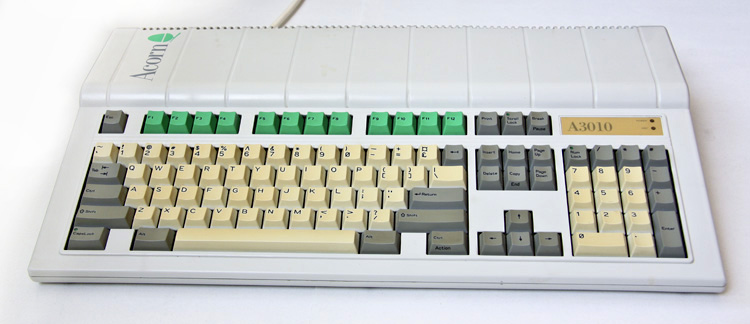
\includegraphics{acorn3010top.jpg}
    \end{center}

    The keyboard in the Acorn A3010 case is very PC-like, it has 12 function
    keys and LEDs for Caps Lock, Scroll Lock and Num Lock.

    The back of the case offers holes for connectors for: one DB-25 parallel, 
    one DB-9 serial, two DB-9 joysticks, one stereo jack, one VGA, one RF and
    ON/OFF switch.

    Also there is a hole in the left side for a reset button, and a disk drive
    bay at the right side.

    At the moment, only the ON/OFF switch, VGA connector, Composite video RCA
    output, and reset button are used.

    \pagebreak
    % ==========================================================================
    \section{I/O Decoding}
    % ==========================================================================

    The Z80 communicates with devices via the Address and Data buses. And then
    the signals \textit{/MREQ} (for memory devices) and \textit(/IORQ) (for I/O
    devices).

    To avoid bus contention\footnote{Bus contention occurs when all devices
    communicate directly with each other through a single shared channel
    (Address and Data buses), and more than one device attempts to place values
    on the channel at the same time.}, we need to enable each device one at a
    time.

    dastaZ80 uses a 74HCT138 (3-to-8 Line Decoder) to allow the CPU to enable
    I/O devices (non-memory devices). The outputs are enabled (low) when /MREQ
    is high, /IORQ is low and A7 is low (i.e. addresses below 0x80). This
    configuration gives 16 addresses for each device (e.g. \texttt{0x00} to
    \texttt{0x0F} for a device attached to output /Y0), for a total of 8 devices.

    \begin{tabular}{| c | c | c | c | c | m{4.5cm} | }
        \hline
        \rowcolor{lightgray}
        A6 & A5 & A4 & 74138 output & Addresses & Device\\
        \hline
        0 & 0 & 0 & /Y0 & \texttt{0x00} - \texttt{0x0F} & For future use\\
        \hline
        0 & 0 & 1 & /Y1 & \texttt{0x10} - \texttt{0x1F} & TMS9918A (VDP)\\
        \hline
        0 & 1 & 0 & /Y2 & \texttt{0x20} - \texttt{0x2F} & For future use\\
        \hline
        0 & 1 & 1 & /Y3 & \texttt{0x30} - \texttt{0x3F} & \textbf{ROM} Page
        (\texttt{0x38})\\
        \hline
        1 & 0 & 0 & /Y4 & \texttt{0x40} - \texttt{0x4F} & For future use\\
        \hline
        1 & 0 & 1 & /Y5 & \texttt{0x50} - \texttt{0x5F} & For future use\\
        \hline
        1 & 1 & 0 & /Y6 & \texttt{0x60} - \texttt{0x6F} & For future use\\
        \hline
        1 & 1 & 1 & /Y7 & \texttt{0x70} - \texttt{0x7F} & For future use\\
        \hline
    \end{tabular}
    
    \pagebreak
    % ==========================================================================
    \section{Memory Decoding}
    % ==========================================================================

    As dastaZ80 has a ROM chip and a RAM chip, the CPU has to decide from which 
    chip to read and to which chip to write. Actually, write operations are only
    applicable to the RAM chip.

    Also, dzOS\footnote{dzOS is the Operating System of dastaZ80.} resides in
    the ROM chip, but at boot the entire OS is copied into RAM so that it can be
    modified by the user. Hence, dastaZ80 needs a way to disable the ROM chip
    after the copy has finished.

    % ==========================================================================
    \subsection{Extra signals}
    % ==========================================================================

    To make the logic even more tight, dastaZ80 uses a 74HCT32 (Quad 2-Input or
    Gates) to create three new signals from signals comming from the Z80 CPU:

    \begin{itemize}
        \item \textit{/WR} or \textit{/MREQ} = \textit{/MEMWR}
        \item \textit{/RD} or \textit{/MREQ} = \textit{/MEMRD}
        \item \textit{/WR} or \textit{/MEMREG\_SEL}\footnote{Output /Y3 from the
        I/O Decoder 74HCT138} = \textit{/MEMREG}
    \end{itemize}

    % ==========================================================================
    \subsection{ROM Paging}
    % ==========================================================================

    The ROM paging (disable the ROM chip and enable the RAM chip for all memory
    related operations) is done with a 74HCT273 (Octal D-type Flip-Flop with
    Clear) acting as a external register, where the output 1 of this chip is 
    defined as \textit{/ROMPAGE}.

    When a 0 or a 1 is put into the register's input D0 and \textit{/MEMREG} 
    becomes high, then \textit{/ROMPAGE} signal becomes low or high.
    
    This 74HCT273 is identified in the circuit as \textit{MEMREGCFG}.
    
    % ==========================================================================
    \subsection{Putting all together}
    % ==========================================================================
    
    At power-on or after reset, the 74HCT273 is reset and all outputs are set to
    low, therefore \textit{/ROMPAGE} becomes low. From now on, when there is a
    memory read (\textit{/MEMRD} low) for an address lower than 0x4000
    (\textit{A14} and \textit{A15} low), the ROM chip is enabled
    (\textit{/ROM\_CE low}). When the address is equal or higher than 0x4000
    (\textit{A14} or \textit{A15} high), the RAM chip is enabled
    (\textit{/ROM\_CE} high).

    When there is an IO write (\textit{/IORQ} and \textit{/WR} low) to the any
    address from 0x30 to 0x3F, \textit{/MEMREG\_SEL} becomes low and therefore 
    \textit{/MEMREG} becomes low and \textit{MEMREG}\footnote{\textit{MEMREG} is
    an inverted signal of \textit{/MEMREG} done via a 74HCT04} becomes high. This
    (\textit{MEMREG} high) triggers the Flip-Flop on the 74HCT273, which takes
    whatever is at the inputs (CPU Data bus: \textit{D0}..\textit{D7}) and
    latches it to the outputs. Thus, if \textit{D0} contains a 1,
    \textit{/ROMPAGE} will go high and stay like that until \textit{MEMREG} goes
    high again. From now on, when there is a memory read (\textit{/MEMRD} low)
    \textit{/ROM\_CE} will be high independently of the address (\textit{A14}
    or \textit{A15}, low or high), thus only enabling the RAM chip.

    \pagebreak
    % ==========================================================================
    \section{Appendixes}
    % ==========================================================================
    \label{sec:appendixes}

    % ==========================================================================
    \subsection{History (Timeline) of dastaZ80}
    % ==========================================================================

    These are the experiences of a guy that had very basic knowledge about
    electronics\footnote{When I started this project, my only knowledge about
    electronics was; Ohm's and Kirchhoff's laws, and some basic understanding
    on how capacitors, diodes and resistors work.} but decided to build his own
    computer from scratch and make an operating system and some software for it.

    \begin{itemize}
        \item \textbf{May 2012}
        \begin{itemize}
            \item I decided to go ahead with my idea of programming an operating
            system, and decided to do it for a computer that I'll build and call
            \textit{DastaZ80}.
            \item I start first designs (in paper) on how to connect CPU to ROM
            and RAM.
        \end{itemize}
        \item \textbf{June 2012}
        \begin{itemize}
            \item First test with a Z80 on a breadboard.
        \end{itemize}
        \item \textbf{July 2012}
        \begin{itemize}
            \item I've put together a breadboard with CPU, ROM, Clock, SIO/0 and
            MAX232, and connected it to a PC through the serial port. Nothing
            appears on the terminal emulator on the PC. It could be a dozen of
            things :-(
        \end{itemize}
        \item \textbf{August-December 2012}
        \begin{itemize}
            \item Frustrating period trying to make the computer work with the
            serial port and not having any luck.
        \end{itemize}
        \item \textbf{January 2013}
        \begin{itemize}
            \item I've built different test circuits. None worked.
        \end{itemize}
        \item \textbf{February 2013}
        \begin{itemize}
            \item I've built a debug board (consisting just of six 7-segment LED
            displays) and connected it to simple circuit (consisting of CPU and
            ROM). I've programmed the ROM with a simple counter program
            (counting from 0 to 15 and then from 15 to 0). The result is quite
            disappointing; it seems the Z80 just reads all instructions, but it
            doesn't execute them, because I've noticed that it doesn't do the
            loops but just reads from 0000h to 00012h (i.e. from start to
            \textit{HALT}). I've tested the CPU on my Amstrad CPC 6128 and it
            works, so I discard the possibility that the CPU doesn't work. No
            idea what's happening, and even worse, no idea what to do. 
            \item After some more tests, I discovered something; I obtain
            different results when I touch/reseat the cables on the breadboard!
            It seems either the cables or the breadboard itself are making false
            connections. This could be the root of the problems I had up until
            now. I have sockets for the Z80 and AT28C64B. I'm going to start
            soldering a basic circuit and test again.
        \end{itemize}
        \item \textbf{September 2014}
        \begin{itemize}
            \item Relocated to another country. Project is halted.
        \end{itemize}
        \item \textbf{May 2019}
        \begin{itemize}
            \item I re-start the project, using an software emulator I made as a
            starting point, so that I can focus on developing the OS.
            \item The Serial Interface with an MC6850B ACIA is now working and I
            can connect to the dastaZ80. The OS is working.
        \end{itemize}
        \item \textbf{July 2020}
        \begin{itemize}
            \item DZOS booting and CLI accepting first commands.
            \item The implementation of the FAT file system has taken most of my
            time, and still I don't have it fully working. It was not fun. I'll
            take a break.
        \end{itemize}
        \item \textbf{May 2022}
        \begin{itemize}
            \item I re-start the project (again). Decided to implement a simpler
            file system that I call dastaZ80 File System (DZFS).
        \end{itemize}
        \item \textbf{June 2022}
        \begin{itemize}
            \item DZFS is working. I can format and catalogue the disk, load
            files into memory and run them.
        \end{itemize}
        \item \textbf{July 2022}
        \begin{itemize}
            \item Thanks to the VGA32 I have VGA output, and thanks to a
            modified version of my Teensy++ 2.0 based keyboard controller for
            Acorn Archimedes A3010 keyboard I have a keyboard working.
            \item I've also designed a backplane to fit temporarily my boards
            inside the A3010 computer case until I make a single board. I
            designed the backplane with EasyEDA and ordered the PCBs at JLCPCB.
            I'm waiting for the PCBs to arrive.
        \end{itemize}
        \item \textbf{August 2022}
        \begin{itemize}
            \item \textit{ROM Paging} implemented. DZOS gets copied to RAM and
            then ROM is disabled.
            \item Backplane boards arrived and works perfectly. Only to take in
            consideration that the CompactFlash board needs to be very close to
            the CPU to work properly. I'll research about buffering bus lines to
            see if it works while putting the CF card a bit far away. I need
            this, because I want to have the CF card accessible at the back of
            the case, so that CF cards can be exchanged.
        \end{itemize}
        \item \textbf{September 2022}
        \begin{itemize}
            \item Mark I fully assembled and working.
            \item I've made a design with EasyEDA for a PCB that contains CPU,
            RAM, ROM, Clock and Reset. It's called the \textit{Main Board}. The
            idea is to free two slots of the Mark I backplane, so that I can fit
            more boards in the future, like for example RTC, VDP. Ordered it at
            JLCPCB. I'm waiting for the PCBs to arrive.
        \end{itemize}
        \item \textbf{October 2022}
        \begin{itemize}
            \item Soldered the components of the Main Board. Some issues on the
            design found, but I managed to make it work with some workarounds.
        \end{itemize}
        \item \textbf{November 2022}
        \begin{itemize}
            \item I've decided to go away from building more (for now) boards.
            Prices of components plus PCBs are too expensive for my taste. I've
            build an Arduino controller (I've called it \textit{Arduino Serial
            Multi-Device Controller (ASMDC)}) that controls the RTC and the SD
            Card (no more CF Card). It communicates with the CPU via serial on
            the SIO/2.
        \end{itemize}
        \item \textbf{December 2022}
        \begin{itemize}
            \item I've added the original Acorn A3010 FDD to ASMDC. It works.
            \item Starting the Mark II by adding a Texas Instruments TMS9918A
            (VDP) for graphics video output.
            \item I designed a board for the TMS9918A that can be tested first
            with Arduino and then easily, just two jumpers, modified to work
            with dastaZ80.
            \item Testing the VDP board with Arduino was successful: 
            \begin{itemize}
                \item At first I was getting good results in text mode, but in
                graphics mode I had no sprites and text lines were duplicated in
                pairs every odd line. For several hours I checked and
                double-checked and triple-checked my circuit and Arduino code.
                I couldn't find the problem. Finally, reading the VDP manual I
                noticed that the nominal current need of the VDP is about 200mA,
                which I'm not sure the Arduino Uno can deliver. I plugged the
                board to a DC-DC converter 5V/2A and all was working. Sprites
                and correct text lines. But a huge rippled image on the screen.
                \item Testing with another power supply brought crispy image.
                It seems those DC-DC step down converters I bought have a big
                voltage ripple on the output.
                \item Also, image on CRT was B/N, due to signal being NTSC. But
                with the addition of a  NTSC-to-PAL converter all looks fine.
            \end{itemize}
            \item Testing the VDP board with the dastaz80 was successful, though
            there are some artifacts on the screen. Looking at the contents of
            the \textbf{VRAM} with the \textit{vramdump} program, I can see that
            in the Colour Table some bytes have the value \textit{0xF1}, which
            is the value I initialised the Colour Table with. So it seems some
            skipping is happening. I added \textit{NOP} instructions, but no
            change so far. And why only happens with the Colour Table?
            \item Found that the VDP needs 2 \si{\micro\second} to read or write
            a byte to its RAM. A \textit{NOP} instruction at 7.3728 Mhz only
            takes 0.54 \si{\micro\second}, so I need at least four \textit{NOP}s.
            Instead I went for creating a subroutine, that with its instructions
            plus the \textit{call} takes 6.24 \si{\micro\second}
        \end{itemize}
    \end{itemize}

    % ==========================================================================
    \subsection{Acknowledgements and Thanks}
    % ==========================================================================

    \begin{itemize}
        \item \textbf{Albert P. Malvino}, for his books \textit{Electronic
        Principles}\cite{malvino1} and \textit{Digital Computer Electronics}
        \cite{malvino2}.
        \item \textbf{M. Morris Mano}, for his book \textit{Computer System
        Architecture}\cite{morrismano1}.
        \item \textbf{Steve Ciarcia}, for his awesome and inspirational book
        \textit{Build your own Z80 computer}\cite{ciarcia1}, which inspired me
        into starting this project.
        \item \textbf{Grant Searle}, for his great \textit{My simple Z80 design}
        \cite{searle1}, which also inspired me to do this project. For his work
        on the NASCOM MS BASIC. And for having the patience to answer all my
        questions.
        \item \textbf{Doctor Volt}, for his \textit{TMS9918 Arduino Library}
        \cite{drvolt}, which allowed me to test my board and finally
        understand how programming the VDP works.
        \item \textbf{David Hansel}, for his \textit{ArduinoFDC Library}
        \cite{dhansel}, which allowed me to add Floppy Disk Drive support.
        \item \textbf{Zilog, Inc.}, for creating the Z80 microprocessor.
        \item \textbf{Gary A. Kildall}, for his CP/M, which inspired my own
        operating system DZOS.
        \item \textbf{My father}, for buying my first computer, an Amstrad CPC
        464, and for teaching me the basics of Z80 assembly language.
    \end{itemize}

    % ==========================================================================
    \subsection{Future Improvements}
    % ==========================================================================

    These are some ideas I have for improvements:

    \begin{itemize}
        \item \textbf{Sound Interface}: stereo sound output with an AY-3-8912.
        \item \textbf{Dual Digital Joystick Port}: Allowing connection of two
        Commodore 64 compatible (because I have a few of them) joysticks.
        \item \textbf{Cartridge Port}: allowing almost instantaneously load and
        access to programs stored in EEPROMs.
    \end{itemize}

    % ==========================================================================
    % Bibliography
    % ==========================================================================
    \pagebreak
    \bibliographystyle{unsrt}
    \bibliography{dastaZ80}
\end{document}